\documentclass[12pt,a4paper]{article}
\usepackage[utf8]{inputenc}
\usepackage[spanish,es-tabla]{babel}
\usepackage{geometry}
\usepackage{graphicx}
\usepackage{multirow}
\usepackage{tabularx}
\usepackage{mathptmx}
\usepackage{fancyhdr}
\usepackage{array}
\usepackage[table]{xcolor}
\usepackage{titlesec}
\usepackage{setspace}
\usepackage{microtype}
\usepackage{lastpage}
\usepackage{booktabs}
\usepackage{enumitem}
\usepackage{amsmath}
\usepackage{amsfonts}
\usepackage{amssymb}

\graphicspath{{images/}{../images/}{./}}

\geometry{
    top=4.7cm,
    bottom=2.5cm,
    left=2.5cm,
    right=2.5cm,
    headheight=3.9cm,
    headsep=0.4cm
}

\setstretch{1.15}
\setlength{\parindent}{0pt}
\setlength{\parskip}{0.45em}
\setlength{\tabcolsep}{4pt}

\titleformat{\section}
  {\normalfont\fontsize{12}{14.5}\bfseries}{\thesection.}{0.6em}{\uppercase}
\titlespacing*{\section}
  {0pt}{1.8ex plus 0.4ex minus 0.2ex}{0.6ex plus 0.2ex}

\titleformat{\subsection}
  {\normalfont\fontsize{11.5}{13.5}\bfseries}{\thesubsection.}{0.5em}{}
\titlespacing*{\subsection}
  {0pt}{1.4ex plus 0.3ex minus 0.1ex}{0.4ex plus 0.1ex}

\titleformat{\subsubsection}
  {\normalfont\fontsize{10.5}{12.5}\bfseries\itshape}{\thesubsubsection.}{0.4em}{}
\titlespacing*{\subsubsection}
  {0pt}{1.1ex plus 0.2ex minus 0.1ex}{0.3ex plus 0.1ex}

\newcolumntype{Y}{>{\centering\arraybackslash}X}
\newcolumntype{L}{>{\raggedright\arraybackslash}X}
\newcolumntype{C}{>{\centering\arraybackslash}X}

\definecolor{headerblue}{RGB}{26, 54, 93}
\definecolor{darkblue}{RGB}{43, 108, 176}
\definecolor{lightgraybg}{RGB}{248, 248, 248}
\definecolor{tableheader}{RGB}{232, 238, 246}

\newcommand{\docCodigo}{TI-SIGE-ENT-F2-004}
\newcommand{\docVersion}{1.0}
\newcommand{\docProceso}{BASE DE DATOS / MODELADO RELACIONAL}
\newcommand{\docElaboracion}{03/09/2026}
\newcommand{\docRevision}{03/09/2026}
\newcommand{\docTitulo}{DISEÑO DE BASE DE DATOS RELACIONAL}
\newcommand{\docOrganizacion}{FACULTAD DE INGENIERÍA EN SISTEMAS, ELECTRÓNICA E INDUSTRIAL}
\newcommand{\docSubOrganizacion}{CARRERA DE INGENIERÍA DE SOFTWARE}

\newcommand{\encabezadofrecuente}{%
    \renewcommand{\arraystretch}{1.15}%
    \noindent\makebox[\textwidth][c]{%
    \begin{tabularx}{\textwidth}{|>{\centering\arraybackslash}m{2.8cm}|Y|>{\centering\arraybackslash}m{4.8cm}|}
        \hline
        \multirow{4}{2.8cm}{\centering\raisebox{-1.15cm}{
\includegraphics[width=2.5cm,height=2.0cm,keepaspectratio]{images/logo.png}}}
        & \textbf{\fontsize{9}{11}\selectfont \docOrganizacion} 
        & \textbf{\fontsize{8}{10}\selectfont CÓDIGO:} \fontsize{8}{10}\selectfont \docCodigo \\
        \cline{3-3}
        & \textbf{\fontsize{8.5}{10.5}\selectfont \docSubOrganizacion} 
        & \textbf{\fontsize{8}{10}\selectfont VERSIÓN:} \fontsize{8}{10}\selectfont \docVersion \\
        \cline{2-3}
        & \textbf{\fontsize{8}{10}\selectfont PROCESO:} \fontsize{8}{10}\selectfont \docProceso 
        & \textbf{\fontsize{8}{10}\selectfont ELABORACIÓN:} \fontsize{8}{10}\selectfont \docElaboracion \\
        \cline{2-3}
        & \textbf{\fontsize{8.5}{10.5}\selectfont \docTitulo} 
        & \textbf{\fontsize{8}{10}\selectfont ÚLTIMA REVISIÓN:} \fontsize{8}{10}\selectfont \docRevision \\
        \hline
    \end{tabularx}%
    }%
}

\pagestyle{fancy}
\fancyhf{}
\fancyhead[C]{\encabezadofrecuente}
\fancyfoot[C]{\fontsize{10}{12}\selectfont Página \thepage\ de \pageref{LastPage}}
\renewcommand{\headrulewidth}{0pt}

\begin{document}

\noindent{\fontsize{10.5}{12.5}\selectfont \textbf{Integrantes:} Heidi Villavicencio \quad$\vert$\quad Steeven Toala \quad$\vert$\quad Nixon Hurtado \quad$\vert$\quad Andrea Vásquez}

\vspace{0.25cm}

\section{Título}
\textbf{Denominación del Entregable:} Diseño de Base de Datos Relacional (Modelo ER, Lógico y DDL) -- Código EDT: 2.4

\section{Introducción}
La integridad referencial y la durabilidad de los datos institucionales son requisitos indispensables en un sistema de gestión de calidad académica. En este entregable se formaliza el diseño integral de la base de datos relacional para el motor PostgreSQL 18. Se presentan el Modelo Entidad-Relación bajo notación Crow's Foot, el esquema lógico normalizado en Tercera Forma Normal (3NF) y el diccionario exhaustivo de las 13 tablas relacionales con sus tipos de datos, llaves primarias, foráneas, restricciones de chequeo y políticas de indexación.

\section{Objetivo}
\subsection{Objetivo General}
Diseñar y estructurar la base de datos relacional institucional del sistema SIGE en PostgreSQL 18, garantizando la consistencia, normalización 3NF y trazabilidad de los datos del SGC.
\subsection{Objetivos Específicos}
\begin{itemize}[leftmargin=1.5em, itemsep=2pt]
    \item Modelar el Diagrama Entidad-Relación conceptual y lógico con las 13 tablas relacionales.
    \item Elaborar el Diccionario de Datos exhaustivo con tipos nativos de PostgreSQL 18 y restricciones de integridad.
    \item Diseñar la estrategia de indexación B-Tree y GIN para acelerar las consultas frecuentes.
\end{itemize}

\section{Alcance}
\subsection{Límites del Entregable (In-Scope)}
\begin{itemize}[leftmargin=1.5em, itemsep=2pt]
    \item 13 tablas relacionales: usuarios, roles, facultades, carreras, periodos, documentos, secciones, actividades, evidencias, observaciones, firmas, catalogos, auditoria.
    \item Restricciones de integridad referencial con borrado lógico y cascada controlada.
\end{itemize}
\subsection{Exclusiones (Out-of-Scope)}
\begin{itemize}[leftmargin=1.5em, itemsep=2pt]
    \item Ejecución física de scripts DDL en el servidor (actividad cubierta en EDT 3.1).
\end{itemize}

\section{Definiciones}
\begin{itemize}[leftmargin=1.5em, itemsep=2pt]
    \item \textbf{PostgreSQL 18:} Sistema de gestión de bases de datos relacional y orientado a objetos open source.
    \item \textbf{Tercera Forma Normal (3NF):} Estado de normalización donde no existen dependencias funcionales transitivas entre atributos no clave.
    \item \textbf{Crow's Foot (Pata de Cuervo):} Notación gráfica estándar para representar cardinalidades en modelos Entidad-Relación.
    \item \textbf{Diccionario de Datos:} Repositorio detallado que describe la estructura, significado y restricciones de cada columna de la base.
\end{itemize}

\section{Responsabilidades}
\begin{itemize}[leftmargin=1.5em, itemsep=2pt]
    \item \textbf{Nixon Hurtado / Steeven Toala (Responsables EDT 2.4):} Diseño del modelo ER, diccionario de datos y definición de constraints.
    \item \textbf{Heidi Villavicencio (Analista):} Verificación de campos obligatorios según formatos SGC.
    \item \textbf{Ing. Paulo Torres (Docente Evaluador):} Aprobación del esquema de base de datos.
\end{itemize}

\section{Normativa Legal y Técnica}
\begin{itemize}[leftmargin=1.5em, itemsep=2pt]
    \item \textbf{ANSI/ISO/IEC 9075:2016 (SQL Standard).}
    \item \textbf{Norma ISO/IEC 25012:2008:} Software engineering -- Data quality model.
\end{itemize}

\section{Método, Políticas y Contenidos}
Se utilizó modelado en 3NF. En la Figura \ref{fig:s2_04_erd} se presenta el Diagrama Entidad-Relación consolidado en notación Crow's Foot.

\begin{figure}[htbp]
    \centering
    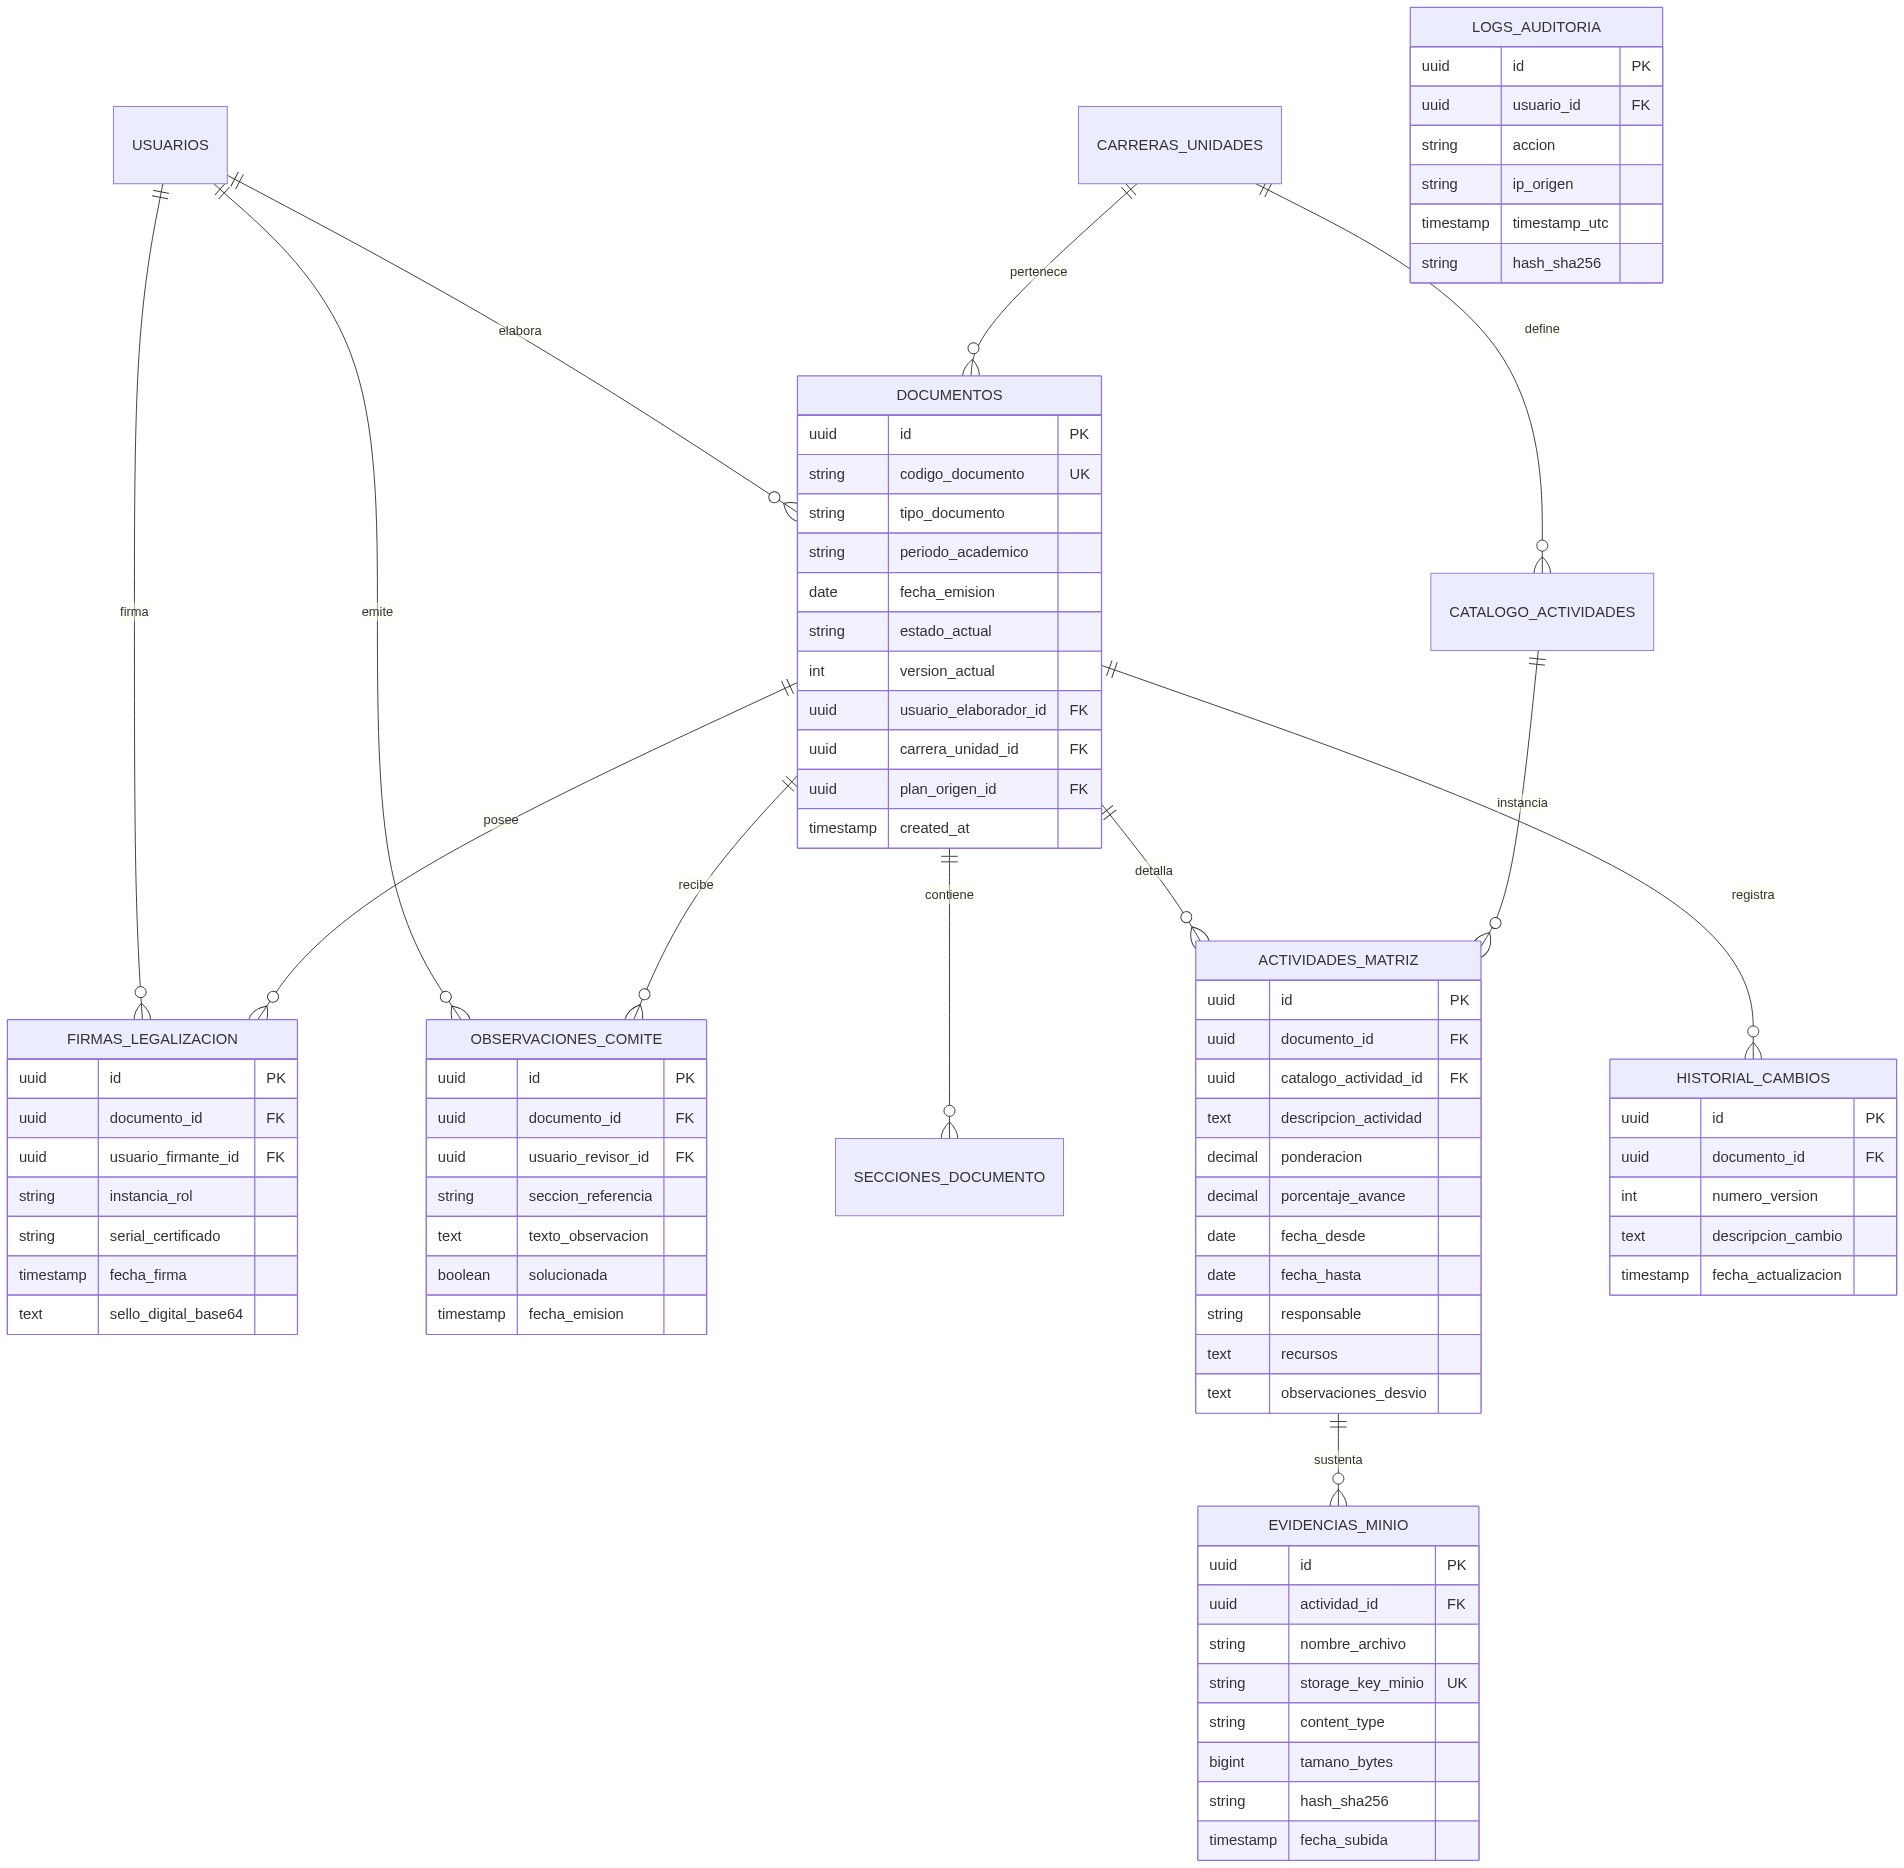
\includegraphics[width=0.88\textwidth,height=5.8cm,keepaspectratio]{images/s2_04_erd_postgresql.png}
    \caption{Diagrama Entidad-Relación Crow's Foot del Sistema SIGE (13 Tablas).}
    \label{fig:s2_04_erd}
\end{figure}

\section{Descripción de actividades}
\subsection{Estructura General de las 13 Tablas Relacionales}
\begin{table}[htbp]
\centering
\small
\renewcommand{\arraystretch}{1.2}
\begin{tabularx}{\textwidth}{|c|>{\bfseries}m{3.2cm}|X|c|}
\hline
\rowcolor{tableheader}
\textbf{No.} & \textbf{Tabla} & \textbf{Descripción y Propósito Institucional} & \textbf{Registros Est.} \\
\hline
1 & \texttt{roles} & Catálogo de roles de seguridad (Docente, Coordinador, Subdecano, Admin). & 4 \\
\hline
2 & \texttt{facultades} & Unidad académica mayor (FISEI). & 1 \\
\hline
3 & \texttt{carreras} & Programas académicos de pregrado de la facultad. & 5 \\
\hline
4 & \texttt{usuarios} & Credenciales institucionales, nombres, email y rol asignado. & 120 \\
\hline
5 & \texttt{periodos\_academicos} & Ciclos semestrales oficiales con fechas límite y fechas extemporáneas. & 10 \\
\hline
6 & \texttt{documentos} & Cabecera de Plan de Trabajo e Informe con estado SGC y código único. & 1,500 \\
\hline
7 & \texttt{secciones} & Contenido de texto enriquecido HTML de cada sección descriptiva del SGC. & 7,500 \\
\hline
8 & \texttt{actividades} & Registro detallado de la Matriz Dinámica con horas, ponderación y avance. & 15,000 \\
\hline
9 & \texttt{evidencias} & Metadatos de anexos en MinIO S3 con URL, tamaño y hash SHA-256. & 25,000 \\
\hline
10 & \texttt{observaciones} & Registro de comentarios de coordinadores a nivel de sección o actividad. & 3,000 \\
\hline
11 & \texttt{firmas\_documento} & Registro del circuito de firmas con cargo, estampa de tiempo y hash. & 4,500 \\
\hline
12 & \texttt{catalogos\_sgc} & Tipologías estandarizadas de actividades de docencia, vinculación e investigación. & 50 \\
\hline
13 & \texttt{auditoria\_logs} & Bitácora inmutable de eventos del sistema para trazabilidad forense. & 100,000 \\
\hline
\end{tabularx}
\caption{Catálogo de Tablas del Esquema Relacional PostgreSQL 18.}
\label{tab:tablas_bd}
\end{table}

\subsection{Diccionario de Datos: Tabla Central \texttt{documentos}}
\begin{table}[htbp]
\centering
\footnotesize
\renewcommand{\arraystretch}{1.15}
\begin{tabularx}{\textwidth}{|>{\bfseries}m{3.2cm}|m{2.5cm}|c|X|}
\hline
\rowcolor{tableheader}
\textbf{Campo (Columna)} & \textbf{Tipo de Dato} & \textbf{Nulo} & \textbf{Restricciones y Claves} \\
\hline
\texttt{id} & \texttt{UUID} & NO & Primary Key (\texttt{gen\_random\_uuid()}) \\
\hline
\texttt{codigo\_documento} & \texttt{VARCHAR(50)} & NO & Unique Key (\texttt{TI-SIGE-PLA-2026-001}) \\
\hline
\texttt{tipo\_documento} & \texttt{VARCHAR(20)} & NO & Check: in ('PLAN\_TRABAJO', 'INFORME\_CUMPLIMIENTO') \\
\hline
\texttt{usuario\_id} & \texttt{UUID} & NO & Foreign Key $\to$ \texttt{usuarios(id)} \\
\hline
\texttt{periodo\_id} & \texttt{UUID} & NO & Foreign Key $\to$ \texttt{periodos\_academicos(id)} \\
\hline
\texttt{estado} & \texttt{VARCHAR(30)} & NO & Check: in ('BORRADOR', 'EN\_REVISION', 'OBSERVADO', 'FIRMADO', 'LEGALIZADO') \\
\hline
\texttt{porcentaje\_avance} & \texttt{NUMERIC(5,2)} & NO & Default: 0.00, Check: entre 0.00 y 100.00 \\
\hline
\texttt{fecha\_creacion} & \texttt{TIMESTAMPTZ} & NO & Default: \texttt{CURRENT\_TIMESTAMP} \\
\hline
\texttt{hash\_inmutable} & \texttt{VARCHAR(64)} & SÍ & Hash SHA-256 generado al firmar \\
\hline
\end{tabularx}
\caption{Diccionario de Datos de la Tabla \texttt{documentos}.}
\label{tab:diccionario_documentos}
\end{table}

\section{Firmas de Responsabilidad}

\noindent
\renewcommand{\arraystretch}{1.2}
\begin{tabularx}{\textwidth}{|>{\raggedright\arraybackslash}m{2.9cm}|>{\raggedright\arraybackslash}X|>{\centering\arraybackslash}m{4.6cm}|>{\centering\arraybackslash}m{2.3cm}|}
    \hline
    \rowcolor{tableheader}
    \textbf{ACCIÓN} & \textbf{NOMBRE Y CARGO} & \textbf{FIRMA} & \textbf{FECHA} \\
    \hline
    \textbf{Elaborado por:} & Heidi Villavicencio\newline Analista de Calidad / UI-UX & \parbox[c]{4.4cm}{\centering\vspace{4pt}
\includegraphics[height=1.5cm,width=4.0cm,keepaspectratio]{images/firma_heidi.png}\vspace{4pt}} & 03/09/2026 \\
    \hline
    \textbf{Revisado por:} & Steeven Toala\newline Líder de Proyecto / Arquitecto & \parbox[c]{4.4cm}{\centering\vspace{4pt}
\includegraphics[height=1.5cm,width=4.0cm,keepaspectratio]{images/firma_steveen.png}\vspace{4pt}} & 03/09/2026 \\
    \hline
    \textbf{Aprobado por:} & Ing. Paulo Torres, Mg.\newline Docente Evaluador -- Gestión Proyectos & \parbox[c]{4.4cm}{\centering\vspace{8pt}\textbf{\textcolor{gray!80}{\scriptsize [ PENDIENTE DE APROBACIÓN ]}}\vspace{8pt}} & \textbf{\textcolor{gray!90}{Pendiente}} \\
    \hline
\end{tabularx}

\vspace{0.4cm}

\section{Control de Cambios}

\noindent
\renewcommand{\arraystretch}{1.2}
\begin{tabularx}{\textwidth}{|>{\hsize=0.45\hsize\centering\arraybackslash}X|>{\hsize=1.55\hsize\raggedright\arraybackslash}X|>{\hsize=1.2\hsize\raggedright\arraybackslash}X|>{\hsize=0.8\hsize\centering\arraybackslash}X|}
    \hline
    \rowcolor{tableheader}
    \textbf{Versión} & \textbf{Descripción del cambio} & \textbf{Responsable del cambio} & \textbf{Fecha de aprobación} \\
    \hline
    1.0 & Emisión inicial del entregable según EDT del Tablero Trello & Equipo de Proyecto SIGE & 03/09/2026 \\
    \hline
\end{tabularx}

\vspace{0.4cm}

\section{Anexos}
\begin{itemize}[leftmargin=1.5em]
\item \textbf{Anexo 1:} Diccionario de Datos Completo de las 13 Tablas en Formato Tabular.
\end{itemize}

\end{document}
